\section*{Magnus Dagon}
\begin{small}
	\begin{wrapfigure}{l}{0cm}
		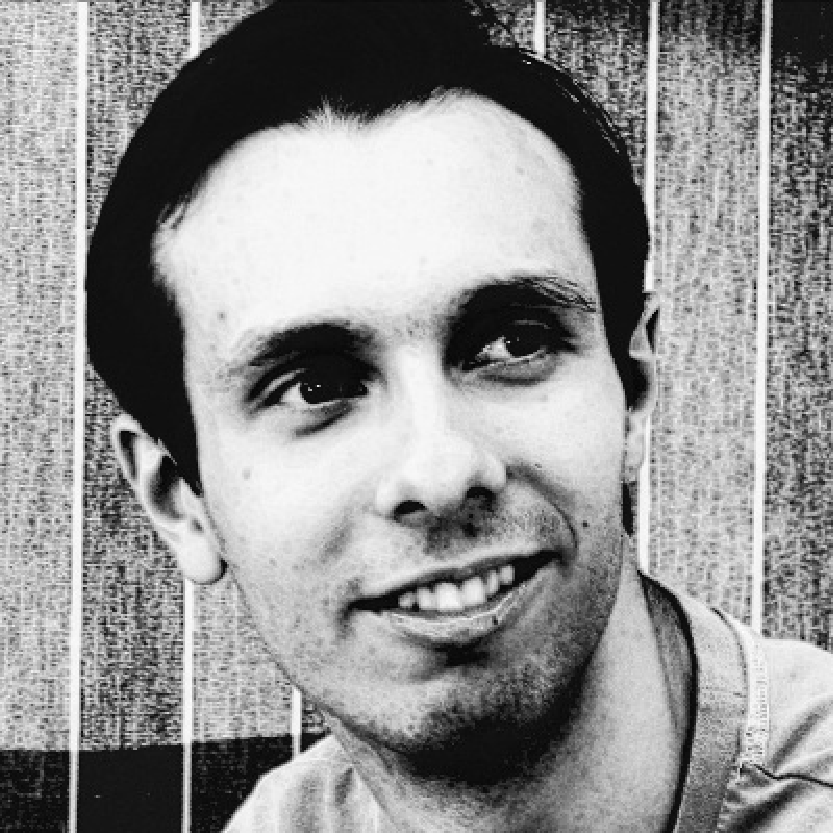
\includegraphics[width=.4\textwidth]{images/magnus_dagon}
	\end{wrapfigure}

	Seudónimo de Miguel Ángel López Muñoz. Nacido en Madrid en 1981. Matemático con un Máster en Criptografía Cuántica y antiguo estudiante de Arquitectura. 

	Su novela corta \emph{El Informe Cronocorp} fue galardonada con el premio UPC en el año 2006 (el certamen de ciencia ficción más importante del país y uno de los mejores dotados a nivel internacional), y poco después fue publicada por Ediciones B. Entre otros premios, ha sido también galardonado en el IX Certamen de Narrativa Corta Villa de Torrecampo en el año 2009, además de finalista en múltiples certámenes. Su primer libro fue \emph{Los Siete Secretos del Mundo Olvidado} (Grupo Ajec, 2010).

	En sus historias suele tener mucha importancia la ambientación, con especial énfasis en lugares misteriosos, apartados o desconocidos. Otorga también mucho valor a los personajes y sus emociones internas, especialmente la soledad y el desarraigo. Aunque tiene múltiples relatos publicados en fantasía y terror (gran parte de ellos englobados bajo un mismo trasfondo al estilo de los Mitos de Cthulhu), ha sido mayormente reconocido por sus obras de ciencia-ficción. Es también conocido por su faceta de ensayista y crítico cinematográfico.

	Además de escritor, es también el cantante y letrista del grupo musical Balamb Garden, que puede escucharse en \url{http://www.balambgardenmusic.blogspot.com/}.
\end{small}

\section*{La obra}
\begin{small}
	\epigraph{
		\lquoti A menudo, cuando leía de adolescente comics de superhéroes, me preguntaba qué sería de Superman, o de Spiderman, si perdieran todo lo que les define como tales. Si, en definitiva, sus peores enemigos les derrotaran sin que hubiera esperanza alguna de recuperar el esplendor perdido. ¿Se hundirían en sus tinieblas? ¿O encontrarían la fuerza interior para convertirse en otra clase de héroes? Este libro trata de abordar la respuesta\rquoti
	}{---Magnus Dagon}

	Los Caídos son una organización formada por antiguos héroes que perdieron sus poderes y, en muchos casos, a sus seres queridos e incluso su identidad. Al caer ellos, el crimen se apodera de Ernépolis~I, la ciudad en la que viven. Pero para contraatacar, deciden crear una organización de muchos hombres que fingen ser uno solo: una silueta negra, con gabardina y sombrero, sólo conocida como El Caído. Desde el punto de vista ciudadano, El Caído es invencible, incluso inmortal. Los enemigos de la ciudad le temen como a una leyenda urbana y le creen un monstruo. Todo ello es parte de un engaño para proteger a la ciudad sin que ella misma sepa que está siendo protegida.

	El mito del superhéroe (y del supervillano) se revisa en este libro para ofrecernos una historia sobre el optimismo, la redención y el espíritu de superación inherente a la condición humana.
\end{small}

\endinput